\documentclass[10pt,xcolor=table]{beamer}

%%%%%%%%%%%%%%%%%%%%%%%%%%% 
%%%%%      TEMA      %%%%%%
%%%%%%%%%%%%%%%%%%%%%%%%%%%
\usetheme{Madrid}                         % tema
\usecolortheme{orchid}                    % cores
\usefonttheme[onlymath]{serif}            % fonte modo matematico

%%%%%%%%%%%%%%%%%%%%%%%%%%% 
%%%%%    PACOTES      %%%%%
%%%%%%%%%%%%%%%%%%%%%%%%%%%

\usepackage[alf]{abntex2cite}             % citações no padrão ABNT
\usepackage[brazil]{babel}                % idioma
\usepackage{Sweave}                       % Sweave
\usepackage{color}                        % controle das cores
\usepackage[T1]{fontenc}                  % codificacao de fontes
\usepackage{graphicx}                     % inclusão de gráficos
\usepackage[utf8]{inputenc}               % codificacao de caracteres
\usepackage{lmodern}
\usepackage{array}
\usepackage{multirow}
\usepackage{enumerate}                    % índices numéricos 
\usepackage{footnote}                     % Lidar com notas de rodapé
\usepackage{booktabs}                     % Tabelas com qualidade de publicação diversas situações
\usepackage{hyperref}                     % para citar hyperlinks da web
\usepackage{adjustbox}
\usepackage{caption}
\newcommand\fnote[1]{\captionsetup{font=small}\caption*{#1}}

%%%%%%%%%%%%%%%%%%%%%%%%%%% 
%%%   INF. DOCUMENTO    %%%
%%%%%%%%%%%%%%%%%%%%%%%%%%%

\title[UFRGS]{Introdução}
\author[Introdução à Econometria]{}

\date{}

\begin{document}
\Sconcordance{concordance:aula1.tex:aula1.Rnw:%
1 252 1}


%%%%%%%%%%%%%%%%%%%%%%%%%%% 
%%%%%     SUMÁRIO     %%%%%
%%%%%%%%%%%%%%%%%%%%%%%%%%%

\begin{frame}
   \titlepage
\end{frame}

\begin{frame}[plain]\frametitle{Sumário}
%\small\tableofcontents
\tableofcontents
\end{frame}

%%%
% OBJETIVOS
%%%

\section{Objetivos}

\begin{frame}\frametitle{Objetivos}
Ao final desta aula os alunos deverão ser capazes de:
  \begin{itemize}
    \item Conhecer alguns campos de atuação da Econometria e sua relação com a teoria econômica;
    \item Diferir sobre Modelos Econômicos e Modelos Econométricos;
    \item Entender o papel dos dados na definição do método econométrico a ser utilizado;
    \item Entender conceitos de Ciência de Dados e sua relação com a Econometria;
    \item Conhecer a plataforma DataCamp que pode ser usada para aprendizagem da linguagem R.
  \end{itemize}
\end{frame}

%%%
% INTRODUÇÃO
%%%

\section{Introdução}

\subsection{Econometria e Teoria Econômica}
\begin{frame}\frametitle{Econometria e Teoria Econômica}
  \begin{itemize}
    \item Por meio da Econometria é possível avaliar empiricamente a teoria econômica:
    \begin{itemize}
      \item Explicar fatos passados;
      \item Testar teorias e hipóteses;
      \item Prever resultados de políticas ou eventos futuros;
      \item Estimar relações entre variáveis econômicas.
    \end{itemize}
    \item Isso é viável porque, em geral, \textbf{há relações de equilíbrio de longo prazo} entre variáveis econômicas.
  \end{itemize}
\end{frame}

\subsection{Econometria e Teoria Econômica}
\begin{frame}\frametitle{Econometria e Teoria Econômica}
  \begin{itemize}
    \item O economista pode fazer uso de diversos campos da econometria de acordo com o \textbf{fundamento econômico}:
    \begin{itemize}
      \item Modelos de Regressão: Regressão Linear Múltipla, Regressão Quantílica, Regressões Penalizadas (Ridge, LASSO, ...)
      \item Modelos de séries temporais (ARIMA, ARCH/GARCH, VAR, VEC, MIDAS, ...)
      \item Modelagem não-paramétrica and semi-paramétrica (Regressão Linear Local, Splines, LOESS, Wavelets, Modelos Aditivos, ...)
      \item Microeconometria (dados em painel, ...)
      \item Macroeconometria (DSGE, DSGE-VAR, ...)
      \item Classificação (Análise Discriminante, ...)
      \item Clustering (K-Means, ...)
      \item Redução da Dimensionalidade (PCA, Análise Fatorial, ...)
      \item Machine Learning e Inteligência Artificial (Redes Neurais, Support Vector Machines, Boosting, Random Forests, Ensemble, ...)
    \end{itemize}
 \end{itemize}
\end{frame}



\subsection{Modelo Econômico}
\begin{frame}\frametitle{Modelo Econômico}
Quais os efeitos do \textbf{treinamento} sobre a \textbf{produtividade} do trabalhador?
\begin{equation}
salárioh = f\left( educ,\quad exper,\quad treina \right)
\end{equation}

onde: 
  \begin{itemize}
    \item $salárioh$ é o salário-hora;
    \item $educ$ representa os anos de educação formal;
    \item $exper$ refere-se aos de experiência no mercado de trabalho;
    \item $treina$ corresponde as semanas ocupadas em treinamento.\\~\\
  \end{itemize}

\textbf{Hipótese:} Os trabalhadores são pagos de acordo com sua produtividade.
\end{frame}

\subsection{Modelo Econométrico}
\begin{frame}\frametitle{Modelo Econométrico} 
Um modelo econométrico para o exemplo anterior
\begin{equation}
salárioh ={\beta}_{0}+{\beta}_{1}educ+{\beta}_{2}exper+{\beta}_{3}treina+u
\end{equation}

em que o termo $u$ contém fatores observados ou não observados, mas que podem influenciar a produtividade, tais como:
  \begin{itemize}
    \item aptidão inata;
    \item qualidade da educação;
    \item formação da família.\\~\\
  \end{itemize}
\textbf{Objetivo:} Testar hipótese sobre o parâmetro ${\beta}_{3}$. Exemplo: ele é diferente de zero?
\end{frame}

\subsection{A Estrutura dos Dados Econômicos}
\subsubsection{Dados de Corte Transversal}

\begin{frame}\frametitle{Dados de Corte Transversal} 

Amostra de indivíduos, empresas, estados, países em um determinado ponto no tempo. Ignoramos o tempo. Tipo de dado mais usado em \textbf{Estatística Econômica}.

  \begin{figure}[hb]
    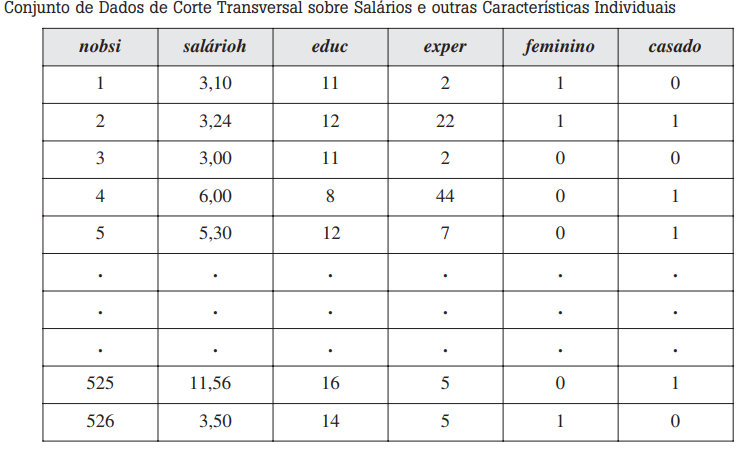
\includegraphics[width=3.5in]{Figure/cortetransversal.png}
  \end{figure}
\end{frame}

\subsubsection{Série Temporal}

\begin{frame}\frametitle{Série Temporal} 

Dados de séries de tempo consistem de observações sobre uma variável ou muitas variáveis ao longo do tempo (preços de ações, IPCA, PIB, Câmbio, Taxa de Juros, ...). Dados mais usados em \textbf{Econometria.} Frequência: intradiária, diária, semanal, mensal, trimestral, anual, etc. 

  \begin{figure}[hb]
    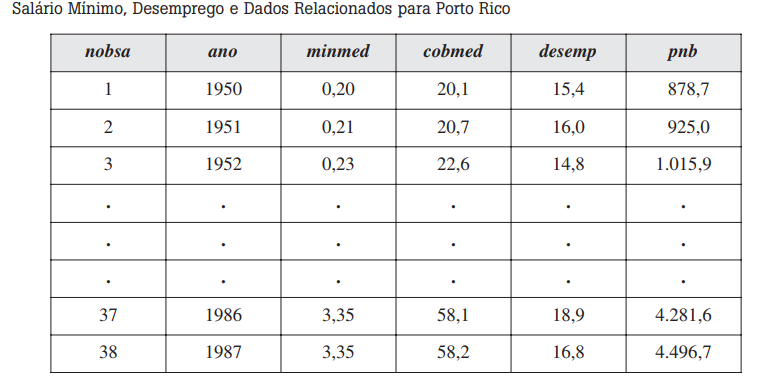
\includegraphics[width=3.5in]{Figure/serietemporal.png}
  \end{figure}
\end{frame}

\subsubsection{Dados em Painel}
\begin{frame}\frametitle{Dados em Painel} 

Um conjunto de dados em painel (ou dados longitudinais) consiste em uma série de tempo para cada variável do corte transversal.  Este tipo de dado costuma ser enfocado em cursos de \textbf{Microeconometria}. Temos as mesmas variáveis do corte transversal ao longo do tempo.

  \begin{figure}[hb]
    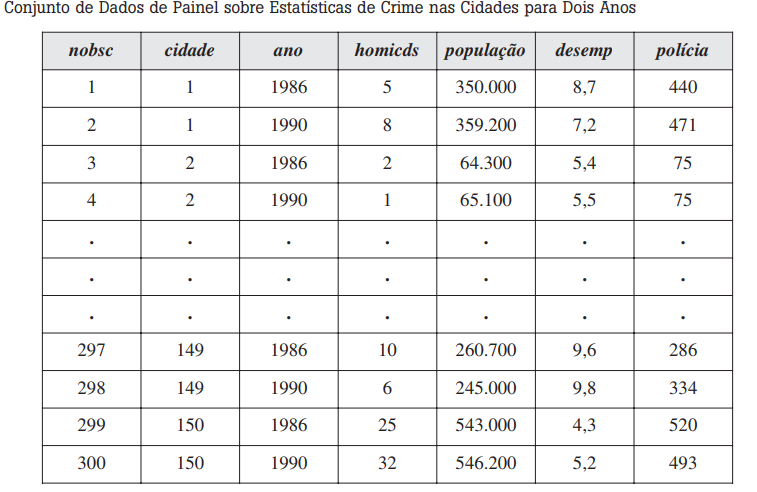
\includegraphics[width=3.5in]{Figure/dadospainel.png}
  \end{figure}
\end{frame}

\subsection{Ciência de Dados}
\subsubsection{Definição}
\begin{frame}\frametitle{Definição} 
  \begin{itemize}
    \item Com a migração para a internet, produzimos um fluxo constante e exaustivo de informação digital;
    \item Estima-se que \textbf{90\% dos dados armazenados no mundo} foram produzidos apenas nos \textbf{últimos dois anos};
    \item Informação tornou-se a moeda mais poderosa e exige que o mercado saiba interpretá-la a seu favor (para gerar valor);
    \item Logo, a profissão de Cientista de Dados se torna crucial;
    \item Áreas de atuação: varejo, saúde, finanças, telecomunicações, segurança, transporte, economia, recursos humanos, ...\\~\\
  \end{itemize}
\textbf{Definição 1}: Ciência de Dados é o termo usado para o processo de extrair \emph{insigths} de dados que são coletados de várias fontes (estruturadas e não estruturadas) \\~\\
\textbf{Definição 2}: Consiste de um conjunto de especialidades, tais como estatística, matemática, programação, computação e \emph{business}
\end{frame}

\subsubsection{Áreas de Conhecimento}
\begin{frame}\frametitle{Áreas de Conhecimento} 
  \begin{figure}[hb]
    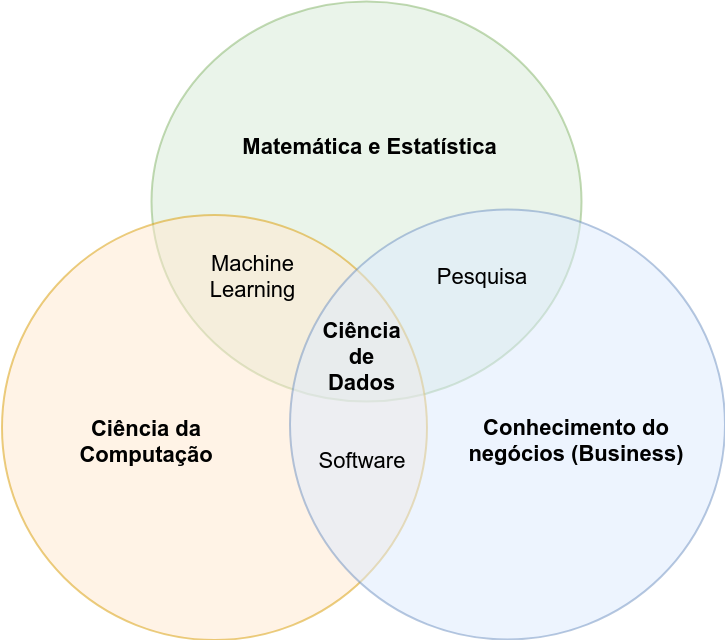
\includegraphics[width=3.5in]{Figure/CientistadeDados.png}
  \end{figure}
\end{frame}

\subsubsection{O Processo de Ciência de Dados}
\begin{frame}\frametitle{O Processo de Ciência de Dados} 
  \begin{enumerate}
    \item Identificar o problema da área de negócio;
    \item Compreender o problema (entidades e atributos);
    \item Coletar conjuntos de dados que representem as entidades;
    \item Limpar e transformar os dados;
    \item Compreender os relacionamentos entre os dados;
    \item Criar modelos estatísticos e matemáticos que representem os relacionamentos;
    \item Utilizar os modelos para fazer predições;
    \item Entregar valor e resultado.
  \end{enumerate}
\end{frame}

\subsection{Big Data}
\subsubsection{Dados Gerados por Minuto}
\begin{frame}\frametitle{Dados Gerados por Minuto} 
  \begin{figure}[hb]
    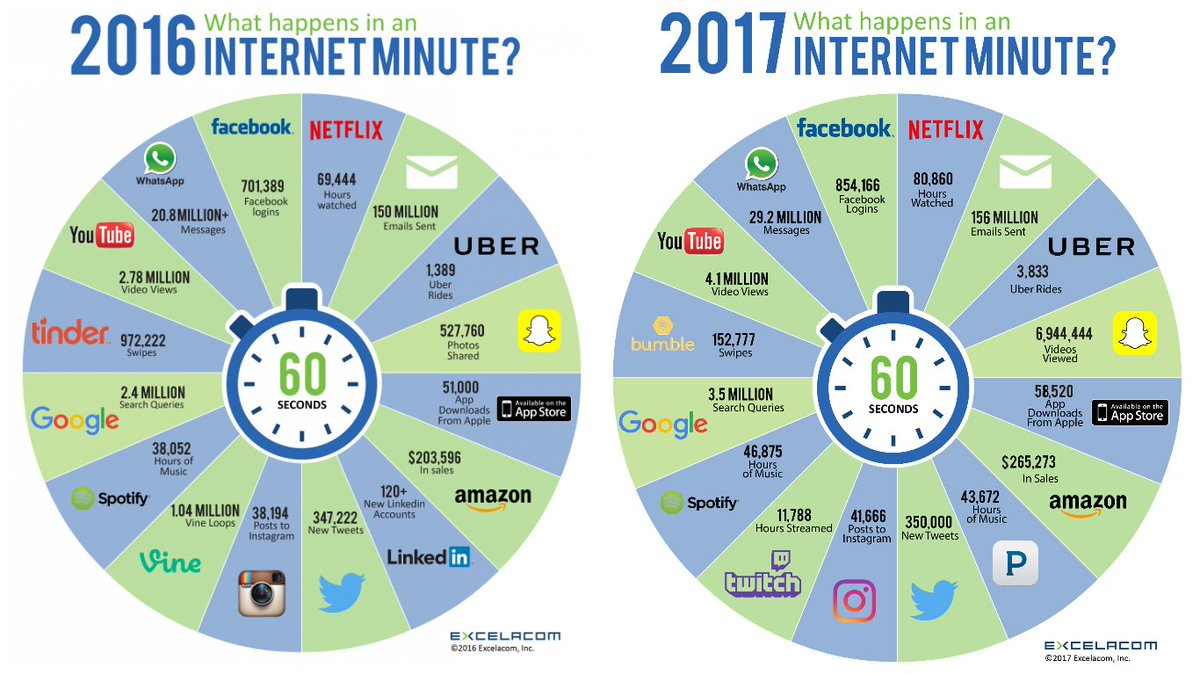
\includegraphics[width=3.5in]{Figure/dataGeneratorByMinuteExcelacom.jpg}
  \end{figure}
\end{frame}

\subsubsection{Velocidade de Crescimento dos Dados}
\begin{frame}\frametitle{Velocidade de Crescimento dos Dados} 
  \begin{figure}[hb]
    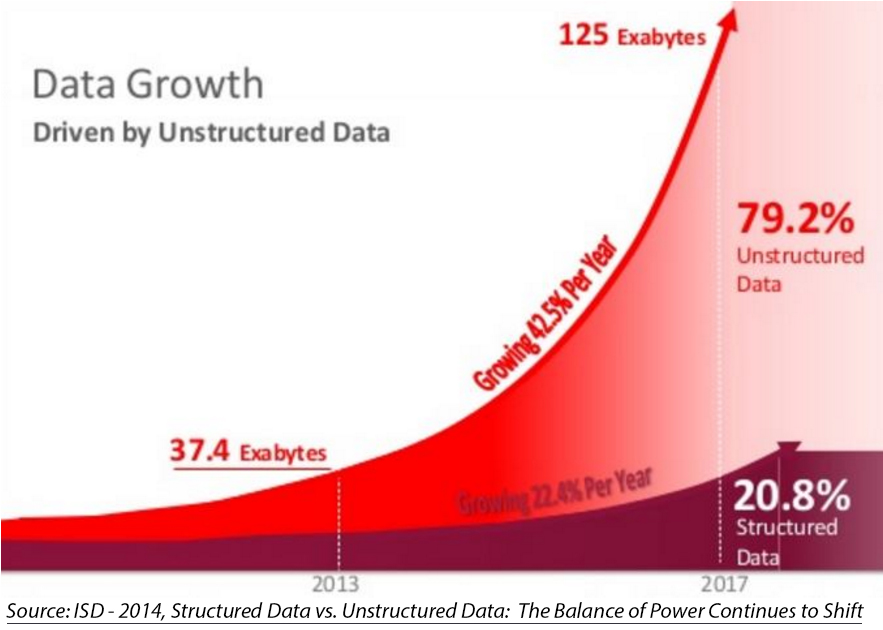
\includegraphics[width=3.5in]{Figure/dataGrowth.jpg}
  \end{figure}
\end{frame}

\begin{frame}\frametitle{Tipos de Dados} 
  \begin{figure}[hb]
    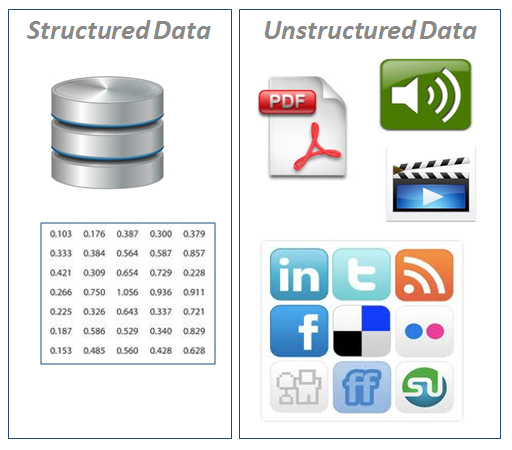
\includegraphics{Figure/datatype.png}
  \end{figure}
\end{frame}

\begin{frame}\frametitle{Economia dos Dados}
\textbf{The Economist:} publicação de 2017 que diz que ter dados atualmente é o mesmo que ter petróleo há 100 anos e que essa nova onda está criando o que os autores chamam de \textbf{Economia dos Dados} \\~\\
  \begin{figure}[hb]
    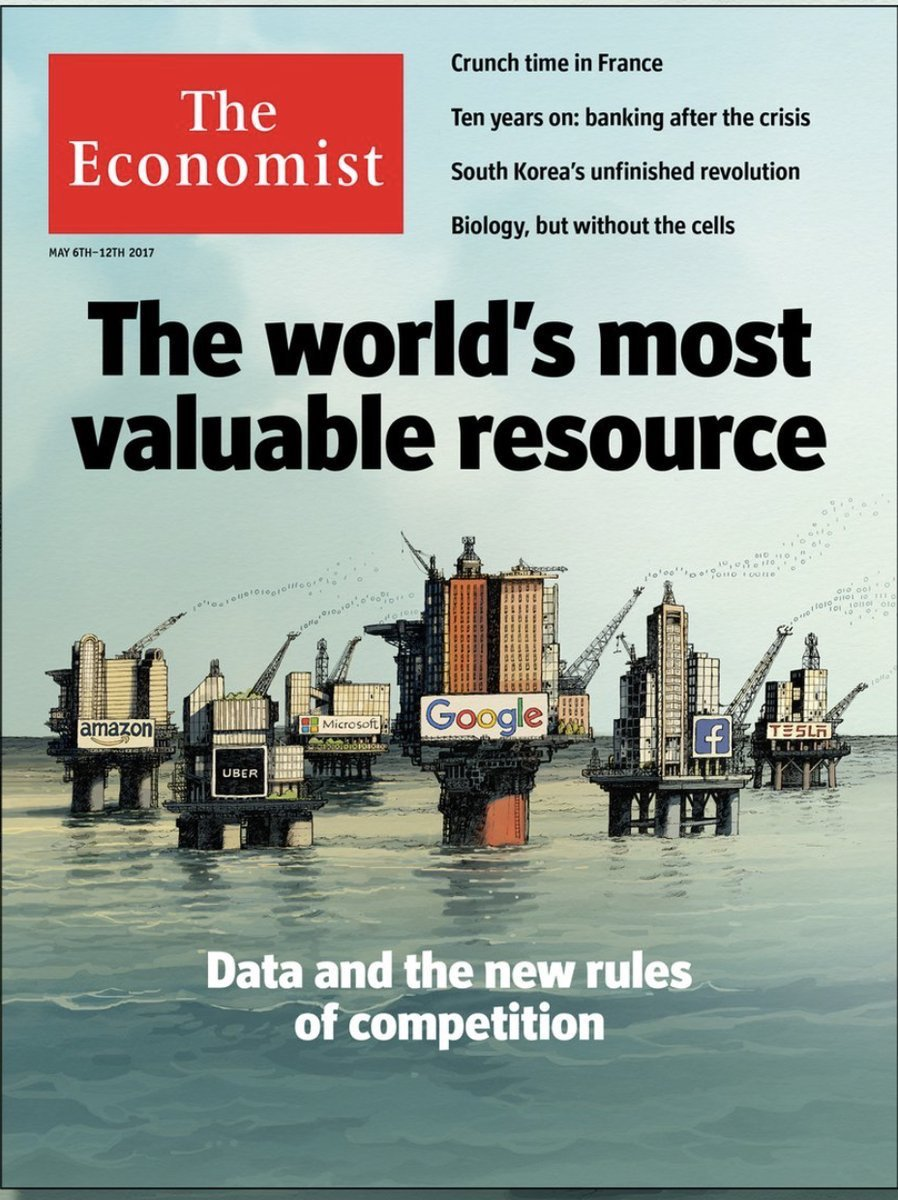
\includegraphics[width=2.5in]{Figure/theeconomist.jpg}
  \end{figure}
\end{frame}


\begin{frame}\frametitle{Cientista de Dados}
\textbf{Harvard Business Review:} publicação de 2012 que abordava o perfil do cientista de dados \\~\\
  \begin{figure}[hb]
    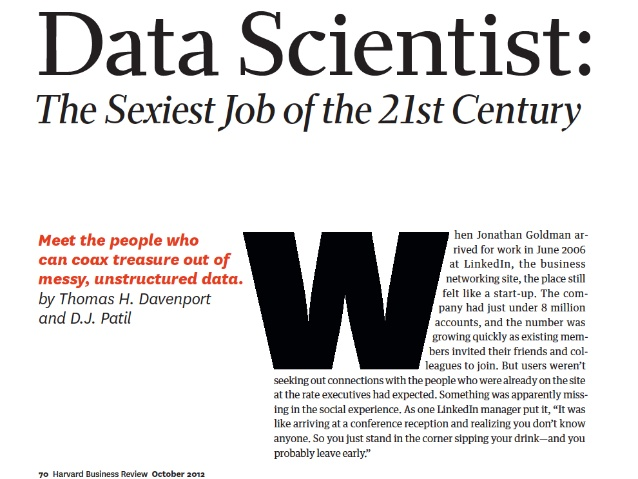
\includegraphics[width=2.5in]{Figure/data-scientist-hbr.jpg}
  \end{figure}
\end{frame}


\end{document}
